\nTitle{Analyse multicritère}

Des deux parties précédentes, émergent 8 propositions de gestion de l'atelier.
Le but de cette partie sera de sélectionner la meilleure solution en fonction des 4 critères préselectionnées.

Ces 4 critères sont :
\begin{itemize}
\item[g1] : bénéfice
\item[g2] : équilibre commercial
\item[g3] : production
\item[g4] : gestion du stock
\end{itemize}

\section{Méthode choisie}

La méthode de résolution choisie sera Électre \rmnum{3} car elle englobe les 2 précédentes.
On pourras ainsi fournir au client la méthode sélectionné comme la plus optimale ainsi qu'une ou plusieurs méthodes alternatives.

Pour réduire au maximum l'échéance, nous avons parallélisé au maximum les flux de travail.
Nous avons donc dès le début du projet commencé à coder sous Matlab un
algorithme de résolution de Électre \rmnum{3} indépendamment des résultats des 2 premières parties.

\section{Algorithme de la méthode}

La réslution des méthodes d'Électre se base sur l'utilisation de deux matrices : la matrice de concordance et la matrice de discordance.
Ces deux matrices confirme ou infirme la superiorité entre deux solutions.

Avant de calculer ces matrices, les notes données dans la matrice de jugement peuvent varié suivant les coéficients attribués aux critère. Ainsi, si un critère à un coéficient 2 fois superieur à un autre, les notes du coéficient le plus important seront répartie sur une echelle plus importante que celles du coefficient le moins important.

Les matrices de concordance et de discordance peuvent être calculé à partir de cette matrice de jugement dont l'echelle des notes dépent des coéficients.

Soit n, le nombre de solutions.
Les matrices de discordances et de concordances seront de taille nxn.\\

Soit la ième et la jème solution, representé par la ième ligne et la jème colonne.\\
En chaque case \{i,j\} de la matrice de concordance, on trouve la valeur confirmant la supériorité de la solution i sur la solution j. Cette valeur est calculé comme la somme des poids des critères dans lesquels i domine j, divisé par la somme des poids de tous les critères.\\
Dans la matrice de discordance, les valeurs infirment de la supériorité de i sur j. Elles sont calculés comme le plus grand écart positif entre les notes de j et les notes de i sur un critère donné.\\

A partir de ces deux matrices et en fonction des seuils de concordances et de discordance, on peut établir le graphe de surclassement.
Pour qu'une solution i soit supérieur à une solution j, la concordance de la supériorité de i sur j doit être superieur au seuil de concordance, et la discordance inferieur ou égal au seuil de discordance.

A partir du graphe de surclassement, il devient facile d'ordonner les solutions.

\section{Mise en œuvre de la méthode}
L'algorithme suivant implémente la méthode Électre \rmnum{3}. À partir de la matrice des jugements, il remet à l'échelle les notes des critères en fonction des poids.

\addCode{../SourcesMatlab/electreSnippet1.m}{matlab}

Puis il calcule les matrices de concordance et de discordance.

\addCode{../SourcesMatlab/electreSnippet2.m}{matlab}


Pour finir, il établit la matrice des surclassement en fonction de ces deux dernières matrices.

\addCode{../SourcesMatlab/electreSnippet3.m}{matlab}

Un graphe est ensuite généré à partir de cette matrice, pour faciliter la lecture.
La meilleur solution apparait alors clairement en tête du graphe, et grâce à la méthode du classement et du classement inverse, on peut obtenir l'ordre des solutions.

\section{Solution proposée}

Dans un premier temps, sans pondérer les critères, on trie les solutions pour en tirer la plus avantageuse. Dans un second temps, on prendras en compte les poids des critères apporté par les résultats de la seconde partie.

\subsection{Sans pondération}

Après quelques tâtonnement, on utilise les seuils de concordance 0,7 et 0,9, et le seuil de discordance 0,4 pour générer un graphe de surclassement le plus clair possible, sans liens superflus.

\begin{figure}[!ht]
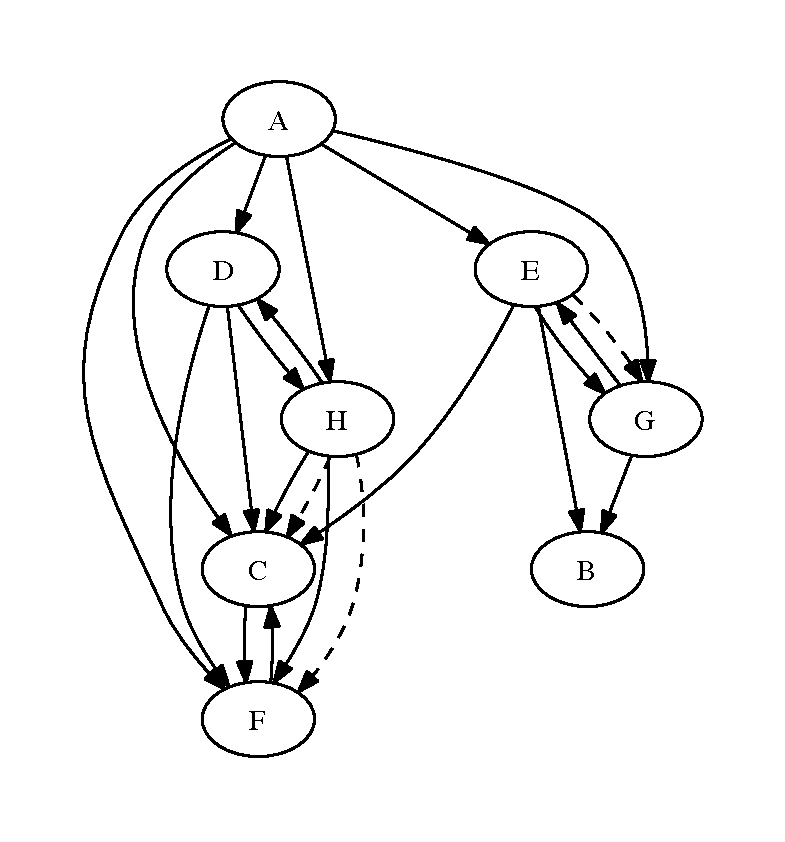
\includegraphics{../SourcesMatlab/electre3-1.pdf}
\caption{Graphe des surclassement sans prise en compte des poids de chaque critère}
\end{figure}

Sur le graphe généré, on voit clairement que la la meilleur solution serait la
solution A car c'est la seule qui n'est dominé par aucune autre.
On voit également que certaines solutions sont équivalentes puisqu'elles se
dominent entres elles. Les couples de solutions \{D, H\}, \{E, G\} et \{C, F\}
sont des couples de solutions équivalentes..
Les solutions F, C et B sont dominés, elles sont donc les moins intéressantes.

\subsection{Avec pondération}

Les pondérations apportés par la partie 2 sont :
\begin{itemize}
\item[g1] : 1.2
\item[g2] : 1.2
\item[g3] : 0.8
\item[g4] : 0.8
\end{itemize}

Sans changer les seuils, le graphe est legèrement modifié, mais on retrouve la solution A en tête.